\begin{tcolorbox}[colback=blue!5!white,colframe=blue!75!black,title=Definición]
	ACA ESCRIBIR LA DEFINICION DE PLCs
\end{tcolorbox}

\subsection{MBE}
\subsection{iFix}
\subsubsection{Guia}
\subsubsection{Programa}


Se realizó una interfaz humana maquina con los siguientes elementos:
	\begin{itemize}
		\item boton de start(acá o en el tablero???)
		\item varias velocidades configuradas previamente
		\item inversión y señalización del mismo
		\item torque???
		\item HMI
        	\subitem Alarmas
       		\subitem Información en tiempo real
        	\subitem Histórico de datos
        	\subitem Control general del banco
	\end{itemize}
	\begin{figure}[htb]
		\centering
		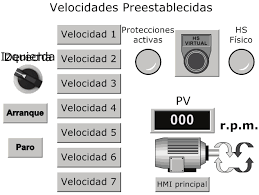
\includegraphics{HMIej.png}
		%\caption{Placa BME280}
		%\label{fig:BME280}
	\end{figure}

\subsubsection{Alarmas- iHistorian}